\section{CPU Results}
\label{sec:MAPS}

\begin{figure}[tp]
    \centering
    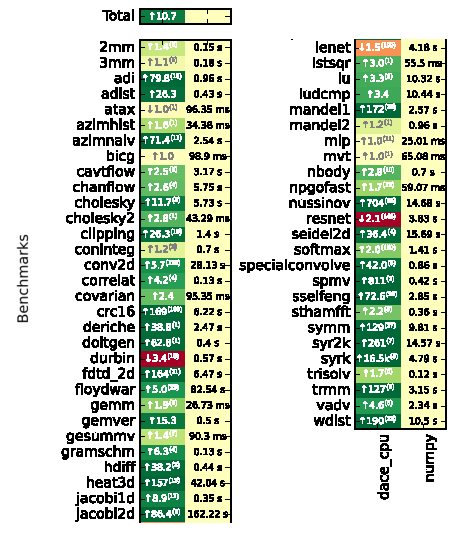
\includegraphics[width=.45\textwidth]{imgs/figure_cpu_crop.pdf}
    \caption{Comparison of DaCe CPU Runtime to NumPy on CPU, showcasing speedup values for DaCe compared to NumPy. The first column number represent the speedup or slowdown factor of the DaCe run compared to the Numpy run. Performance improvements are highlighted in green and uparrows $\uparrow$, while performance degradation is indicated in red (or orange) and downarrows $\downarrow$ for each benchmark.}
    \label{fig:heatmap_cpu}
\end{figure}

We successfully reproduced a total of 56 CPU benchmarks on our Azure cluster, and the results are visualized in Figure~\ref{fig:heatmap_cpu}. In general, DaCe's performance closely matches that reported in the original work~\cite{dace2021}. Notably, in specific cases such as \texttt{heat3d}, \texttt{mandel1}, and \texttt{spmv}, DaCe demonstrates a remarkable performance improvement, achieving speedups of up to 100 times compared to NumPy. On the other hand, benchmarks like \texttt{atax}, \texttt{bicg}, and \texttt{durbin} do not exhibit such substantial enhancements.

Furthermore, this work includes a few additional benchmarks which were not included in \cite{dace2021}, such as \texttt{lstsqr}, \texttt{specialconvolve}, and \texttt{wdist}. While the performance of these benchmarks is undocumented in the original work, our experimental results demonstrate that DaCe can indeed deliver performance improvements for these newly introduced benchmarks.
% We reproduced a total of 56 CPU benchmarks on our Azure cluster, and the results are presented in Figure~\ref{fig:heatmap_cpu}. Generally, the performance of DaCe is similar to that reported in the original work~\cite{dace2021}. In some cases, such as \texttt{heat3d}, \texttt{mandel1}, and \texttt{spmv}, DaCe exhibits a significant improvement of up to 100x compared to NumPy, while benchmarks like \texttt{atax}, \texttt{bicg}, and \texttt{durbin} do not achieve such notable enhancements. On the other hand, few benchmarks such as \texttt{lstsqr}, \texttt{specialconvolve} and \texttt{wdist} are presented in this work but not included in \cite{dace2021}. Although the results is unknown in \cite{dace2021}, our experimental result reveals that DaCe could provide performance improvement on the newly introduced benchmarks.

Benchmarks that experience significant speedup in DaCe typically involve operations performed on arrays, allowing DaCe to optimize them by leveraging OpenMP for parallel execution. Furthermore, applying the Stateful Dataflow multiGraphs~\cite{SDFG} model to the calculations enables further optimization of the data flow, resulting in improved performance.

On the other hand, benchmarks such as \texttt{lenet}, \texttt{resnet}, and \texttt{durbin} are unable to benefit from the aforementioned optimizations for higher performance. The performance degradation observed in \texttt{lenet} and \texttt{resnet} is due to the representation of convolutions. The implementation of convolutions in DaCe is translated into multiple atomic operations, resulting in decreased performance compared to other benchmarks. Such observations are also mentioned in the original work~\cite{dace2021}.
Regarding the \texttt{durbin} benchmark, the implementation utilizes \texttt{dace.map} to explicitly parallelize the \texttt{flip()} computation.  Nontheless, in this specific case, the problem size is not sufficient to offset the overhead of parallelization. By explicitly configuring \texttt{OMP\_NUM\_THREADS} to 8, reducing the parallelism, DaCe can achieve a performance improvement of 2x compared to NumPy.

In the DaCe framework, parametric parallelism is supported to enable Python loops to be executed in parallel. There are two ways to take advantage of this feature. First, DaCe provides the LoopToMap transformation, which detects for-loops in the intermediate representation (IR) and uses symbolic affine expression analysis to validate the safety of parallel execution of iterations. Second, DaCe also offers explicit parallelism declaration through map scopes (\texttt{dace.map}), allowing programmers to identify data dependencies based on their knowledge.

Our reproduced results demonstrate that by replacing the Python built-in \texttt{range} iterator with \texttt{dace.map} in the \texttt{syrk} benchmark, the execution time can be significantly optimized, achieving a speedup of 16.5k times compared to NumPy and 30x faster than the original DaCe benchmark. This enhancement also extends to GPU performance. These findings highlight the importance of a programmer's effort in achieving optimal performance. If a programmer can accurately identify data dependencies, the benefits will be much greater than those achieved through the automatic LoopToMap transformation.